\chapter{Struttura del software}

\section{Linguaggi e librerie}
L'applicazione ha come \textit{target platform} \textit{Android} perci\`o il linguaggio usato principalmente \`e stato \textit{Java}. Da notare che su \textit{Android} il linguaggio \`e presente nella versione 7, perci\`o non sono disponibili alcune funzionalit\`a di Java 8 come i metodi di default, \textit{stream}, \textit{lambda expression} ecc. Sono state usate delle librerie esterne fra i quali \textit{Gson} che consente la serializzazione/de-serializzazione dei dati, \textit{lombok} che fornisce delle annotazioni che abbreviano il codice mantenendo una buona espressivit\`a, varie librerie di supporto Android ed una libreria \textit{Apache} che fornisce molte utilit\`a matematiche. Mosso dalla curiosit\`a, ho provato ed alla fine utilizzato nel progetto \textit{Kotlin}, un linguaggio che compila in \textit{bytecode} per la JVM $100 \%$ interoperabile con \textit{Java} 6 $(e successivi)$ che, fra le varie cose, fornisce le funzionalit\`a sopracitate mancanti a \textit{Java} 7.

\section{Applicazione}
L'applicazione ha lo scopo di catturare le onde magnetiche all'interno di un edificio tramite il magnetometro, un sensore presente ormai su tutti gli \textit{smartphone}. A livello di codice, per poter ricevere le onde magnetiche dal magnetometro \`e necessario una istanza della sottoclasse \textit{SensorListener} od una classe anonima, che vuol dire creare un'implementazione dei metodi astratti dell'interfaccia sul momento. Il termine anonima deriva dal fatto che, a differenza delle sottoclassi, non viene assegnato un tipo nominale esplicitamente da parte del programmatore. L'istanza sottotipo di \textit{SensorListener} viene poi data input ad una funzione della libreria \textit{Android} che invier\`a  tramite notifiche \textit{push} le onde magnetiche rilevate dal magnetometro alla nostra classe. La scelta tra le due opzioni \`e ricaduta sull'implementazione di una sottoclasse di \textit{SensorListener} perch\'e la logica che ci sta dietro \`e abbastanza avanzata per una classe anonima. Il codice che implementa l'interfaccia  \`e il seguente:
\lstinputlisting[language=Java]{code/sensorlistener.java}
Sono state omesse alcune parti per non allungare ulteriormente il codice e concentrarci sulla parte essenziale della classe. Il metodo \textit{onSensorChanged} viene chiamato da \textit{Android} quando rileva un cambiamento nel campo magnetico. La condizione dentro l'\textit{if} ci permette di registrare le onde magnetiche ad intervalli regolari a patto che \textit{recordingRate} sia diverso da $-1$ (che rappresenta la  disattivazione della registrazione di onde ad intervalli regolari).
\\\\
Questo codice viene utilizzato sia durante la scansione dell'ambiente, cio\`e quando viene costruita per la prima volta la mappa delle distorsioni magnetiche all'interno dell'edificio, sia quando effettuiamo la ricerca della posizione dentro l'edificio.
\\\\
Ad ogni onda magnetica registrata viene assegnata un'etichetta, ovvero un numero intero rappresentante una zona della mappa che stiamo scansionando. Visto che in un secondo vengono raccolte molte onde magnetiche, quando ne abbiamo un numero abbastanza grande si creano delle \textit{fingerprint} che identificano un singolo punto della zona. Di solito un'etichetta identifica un'area (in genere una stanza) rispetto alla \textit{fingerprint} che rappresenta un singolo punto.
\\\\
Appena i dati sono stati raccolti, inizia la fase di preprocessamento dei dati. In questo caso non \`e stata fatta una normalizzazione/standardizzazione dei valori degli attributi perch\'e, tramite test empirici si \`e verificato che, portava ad una accuratezza pi\`u  bassa del $20\%$ circa. Da ogni \textit{fingerprint} sono state estratte nuove caratteristiche di natura statistica, tra le quali: Media, Varianza, Deviazione standard, Mediana, Media troncata, Coefficiente di variazione, Massimo, Minimo, $ 1^{\circ}, 5^{\circ}, 95^{\circ}, 99^{\circ} $ percentile, $ 1^{\circ}, 2^{\circ}, 3^{\circ} $ quartile.
Dopo non abbiamo una fase di addestramento del modello perch\'e nel codice su dispositivo \text{Android} \`e stato usato il \textit{knn} e quindi c'\`e direttamente la fase di ricerca della posizione, od in termini pi\`u  tecnici per quanto riguarda l'apprendimento automatico, la predizione dell'etichetta.
\\\\
Adesso vediamo alcune statistiche sul codice \textit{Java}: il numero di righe \`e pari a 1443 linee di codice in 43 file quindi 43 classi od interfacce mentre con kotlin sono state scritte 742 linee di codice in 16 file.


\section{UML del codice}
Vediamo adesso un diagramma delle classi del codice \textit{Android} sviluppato. Sono state omesse alcune classi dall'UML perch\'e futili al fine di comprendere la struttura del programma.

\begin{figure}[H]
	\centering
	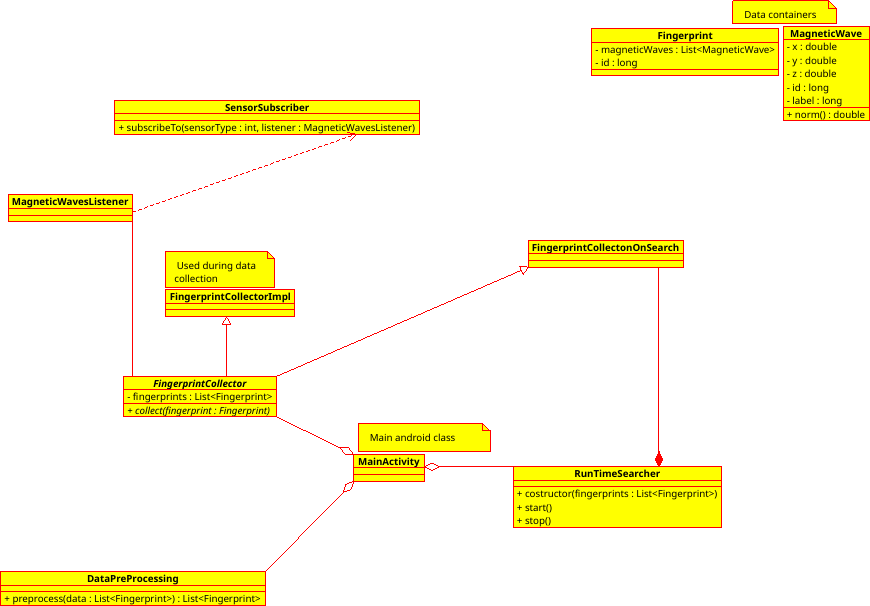
\includegraphics[width=1\linewidth]{img/class_diagram}
	\caption{Diagramma delle classi dell'applicazione}
	\label{fig:classdiagram}
\end{figure}

Al centro abbiamo la \textit{MainActivity}, che rappresenta per lo sviluppatore il "\textit{main}" del programma. In realt\`a non si tratta di una singola funzione di partenza, ma di tante che si attivano come reazione a certi eventi. Abbiamo fra le varie \textit{onCreate} che viene invocata all'avvio del programma, \textit{onPause, onResume} che si fanno intuire dal nome. \`E possibile trovare pi\`u informazione sulla vita dell'\textit{Activity} qua \footnote{\url{https://developer.android.com/reference/android/app/Activity.html}}
Dalla \textit{MainActivity} partono 3 rami, ovvero 3 classi che compongono quest'ultima di cui uno per la raccolta di onde magnetiche, uno per il \textit{preprocessing} dei dati e l'ultimo per la ricerca della posizione dell'utente. In alto a destra invece abbiamo i 2 "contenitori dati" usati in tutto il programma.

\section{Interfaccia grafica}
L'interfaccia \`e stata realizzata ai fini di test pratici delle funzionalit\`a finali dell'applicazione quindi non ha una grande cura da un punto di vista estetico come vedremo pi\`u  avanti.
La parte alta contiene delle \textit{label} raffiguranti i 3 valori catturati tramite il magnetometro e presi tramite le API di Android. \\
Nel mezzo ci sono dei pulsanti per:
\begin{itemize}
	\item Iniziare/Terminare la scansione dell'ambiente.
	\item Incrementare la \textit{label} che viene assegnata alla prossima \textit{fingerprint} registrata. Il \textit{click} di questo bottone dovrebbe avvenire quando vogliamo cambiare zona da analizzare.
	\item Iniziare/Terminare la ricerca.
	\item Serializzare tutti i dati registrati finora
	\item De-serializzare i dati salvati in un \textit{JSON}.
\end{itemize}
Nella parte bassa invece c'\`e una \textit{textbox} contenente il \textit{log} che viene stampato durante l'esecuzione del programma.

\begin{figure}[H]
\centering
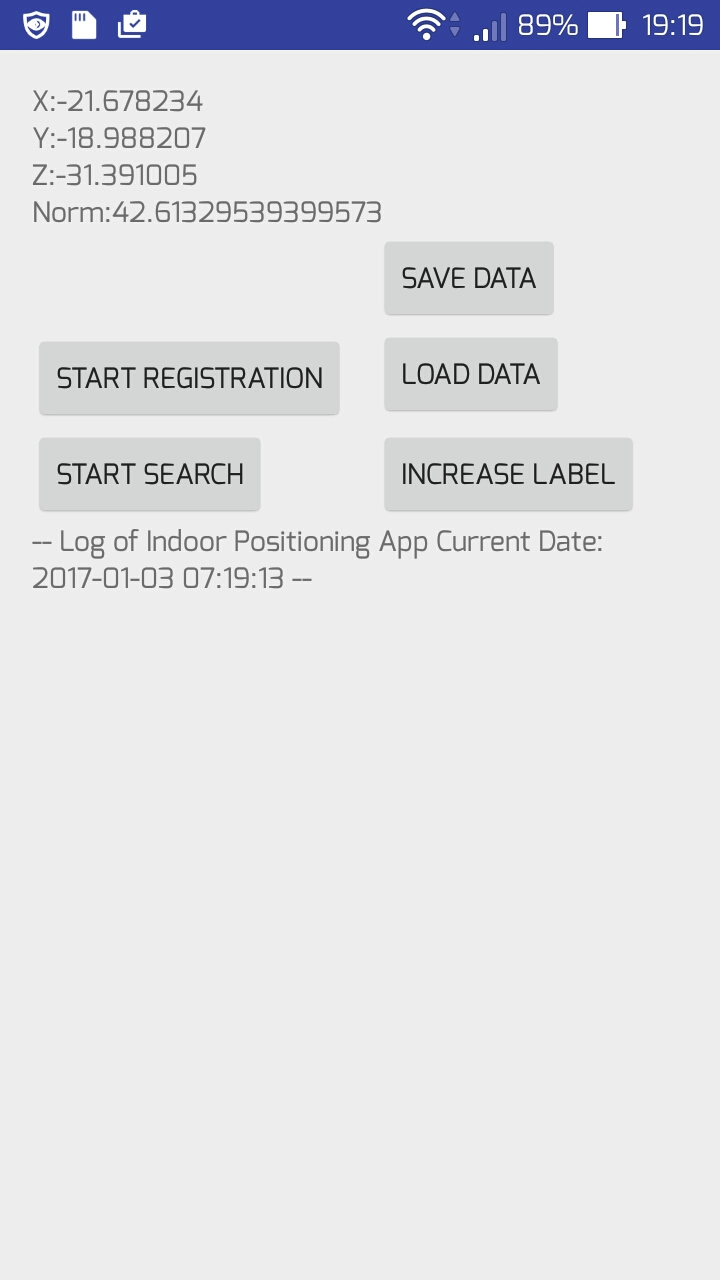
\includegraphics[width=0.4\linewidth]{img/app_screen}
\caption{Interfaccia grafica all'avvio dell'applicazione}
\label{fig:app_screen}
\end{figure}

\begin{figure}
	\centering
	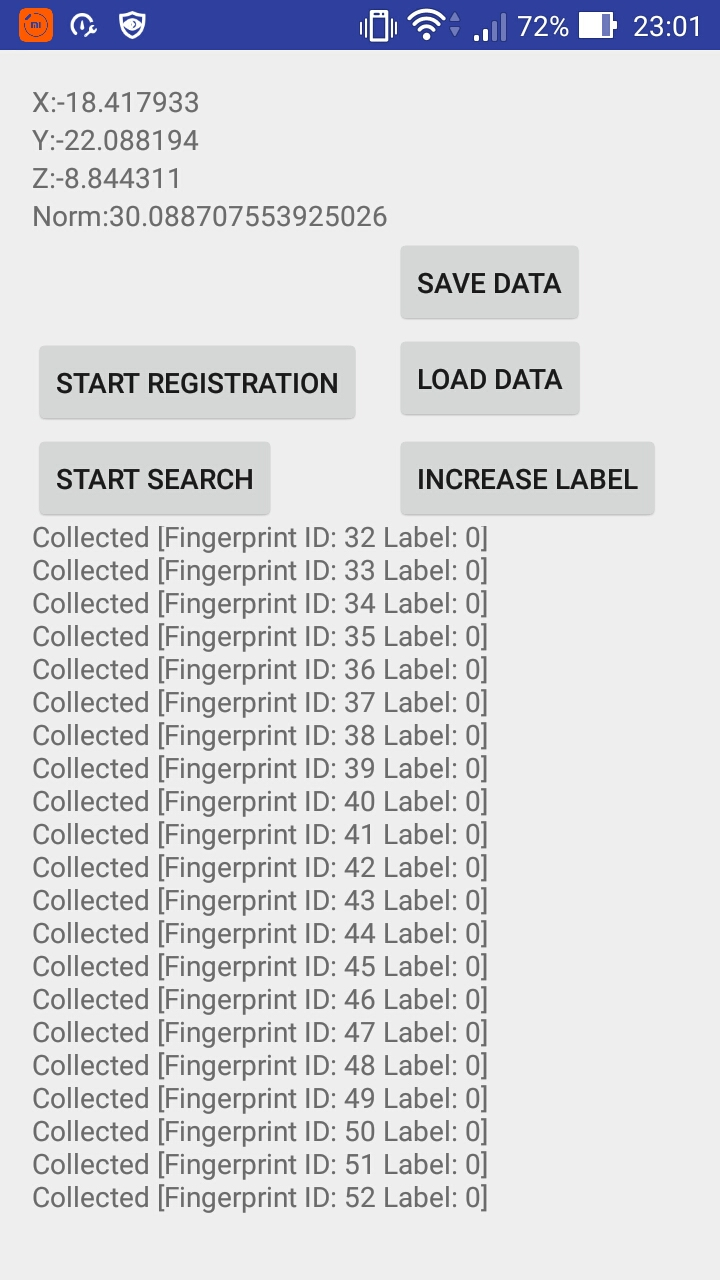
\includegraphics[width=0.4\linewidth]{img/app1}
	\caption{Immagine dell'applicazione durante la raccolta dati}
	\label{fig:app1}
\end{figure}

\begin{figure}
	\centering
	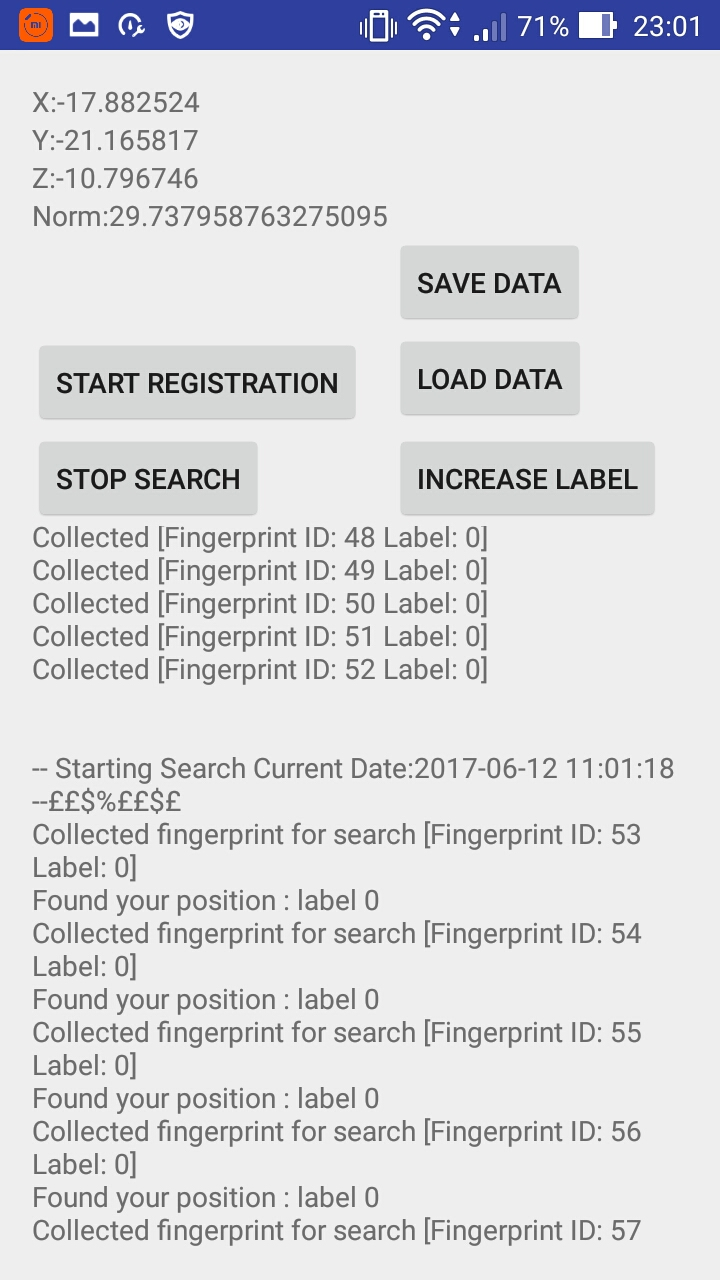
\includegraphics[width=0.4\linewidth]{img/app2}
	\caption{Immagine dell'applicazione durante la ricerca della posizione}
	\label{fig:app2}
\end{figure}


\section{Persistenza dei dati}
Innanzitutto spieghiamo che cos'\`e la serializzazione: \`e una procedura che consente di salvare su supporti di memorizzazione (hard disk, chiavetta usb) dei dati della nostra applicazione mentre la de-serializzazione \`e il procedimento inverso.
L'applicazione consente anche di serializzare tutti i dati registrati fino a quel momento nel formato standard \textit{JSON} tramite la libreria \textit{gson} che fornisce delle funzioni  per il linguaggio \textit{Java} per la serializzazione/de-serializzazione di oggetti. Il file viene salvato nella cartella dati dell'applicazione non visibile all'utente.

\section{Struttura del codice e design pattern}
Nello sviluppo del software sono stati applicati vari \textit{design pattern} visti durante i vari corsi e principi di programmazione. Fra questi ultimi abbiamo il \textit{dependency inversion principle}, \textit{open closed principle}. Riguardo i \textit{design pattern}, sono stati usati frequentemente l'\textit{observer}, il \textit{template} e \textit{factory}.

